
\RequirePackage{fix-cm}
%
%\documentclass{svjour3}                     % onecolumn (standard format)
%\documentclass[smallcondensed]{svjour3}     % onecolumn (ditto)
\documentclass[smallextended]{svjour3}       % onecolumn (second format)
%\documentclass[twocolumn]{svjour3}          % twocolumn
%


\smartqed  % flush right qed marks, e.g. at end of proof
%
\usepackage{graphicx}
\usepackage{balance}
\usepackage{amssymb,amsmath}
\usepackage{wrapfig}
\usepackage{multirow}
\usepackage{graphicx}
\usepackage{algorithm}
\usepackage{algorithmic}
\usepackage{times}
\usepackage{verbatim}

\usepackage{cite}
\usepackage{fancybox}
\usepackage{color}
\usepackage{array}
\usepackage{subfigure}
\usepackage{epstopdf}
\usepackage{booktabs}
\usepackage{caption,fixltx2e}
\usepackage[flushleft]{threeparttable}
%\usepackage{subfig}
%\usepackage{xspace}
\usepackage[hyphens]{url}
\usepackage[hidelinks]{hyperref}
\hypersetup{breaklinks=true}
\urlstyle{same}
\def\UrlBreaks{\do\/\do-} %to break the urls, all in one line

%\newcommand{\ian}[1]{\textcolor{blue}{{\it [Ian says: #1]}}}

\newcommand{\conclusionbox}[1]{%
	\vspace{2mm}
	\framebox[0.45\textwidth][c]{%
		\parbox[b]{0.42\textwidth}{%
			{\it #1}
		}
	}
	\vspace{2mm}
}


\newcommand{\ian}[1]{\textcolor{blue}{{\it [Ian: #1]}}}
%
% \usepackage{mathptmx}      % use Times fonts if available on your TeX system
%
% insert here the call for the packages your document requires
%\usepackage{latexsym}
% etc.
%
% please place your own definitions here and don't use \def but
% \newcommand{}{}
%
% Insert the name of "your journal" with
% \journalname{myjournal}
%
\begin{document}

\title{Empirical Study on the Discrepancy between Performance Testing Results from Virtual and Physical Environments}

%\subtitle{Do you have a subtitle?\\ If so, write it here}

\titlerunning{Discrepancy between Performance Testing Results between diff. environments}        % if too long for running head

\author{Muhammad Moiz Arif \and Weiyi Shang \and Emad Shihab
}

%\authorrunning{Short form of author list} % if too long for running head

\institute{Muhammad Moiz Arif , Weiyi Shang, Emad Shihab\at
              Department of Computer Science and Software Engineering\\
		Concordia University\\
			Montreal, Quebec, Canada\\
              \email{\{mo\_ari, shang, eshihab\}@cse.concordia.ca} }   

\date{Received: date / Accepted: date}


\maketitle

\makeatletter
\def\ps@headings{%
\def\@oddfoot{\scriptsize \hfill \thepage }%
\def\@evenfoot{\scriptsize \thepage \hfill}}
\makeatother
\pagestyle{headings}

\begin{abstract}
Large software systems often undergo performance tests to ensure their capability to handle expected loads. These performance tests often consume large amounts of computing resources and time since heavy loads need to be generated. Making it worse, the ever evolving field requires frequent updates to the performance testing environment. In practice, virtual machines (VMs) are widely exploited to provide flexible and less costly environments for performance tests. However, the use of VMs may introduce confounding overhead (e.g., a higher than expected memory utilization with unstable I/O traffic) to the testing environment and lead to unrealistic performance testing results. Yet, little research has studied the impact on test results of using VMs in performance testing activities. 

To evaluate the discrepancy between the performance testing results from virtual and physical environments, we perform a case study on two open source systems -- namely Dell DVD Store and CloudStore. We conduct the same performance tests in both virtual and physical environments and compare the performance testing results based on the three aspects that are typically examined for performance testing results: 1) individual performance metrics (e.g. CPU Time from virtual environment vs. CPU Time from physical environment), 2) the relationship among performance metrics (e.g. correlation between CPU and I/O) and 3) performance models that are built to predict system performance. Our results show that 1) individual performance metrics from virtual and physical environments do not follow the same distribution hence practitioners cannot simply use a scaling factor to compare the performance between environments,  2) correlations among performance metrics in virtual environments are different from those in physical environments 3) statistical models built based on the performance counters from virtual environments are different from the models built from physical environments suggesting that practitioners cannot use the performance testing results across virtual and physical environments. In order to assist the practitioners leverage performance testing results in both environments, we investigate ways to reduce the discrepancy. We find that such discrepancy can be reduced by normalizing performance metrics based on deviance. Overall, we suggest that practitioners should not use the performance testing results from virtual environment with an simple assumption of straightforward performance overhead. Instead, practitioners should consider leveraging normalization techniques to reduce the discrepancy before examining performance testing results from virtual and physical environments.

\end{abstract}

\section{Introduction}

Software performance assurance activities play a vital role in the development of large software systems. These activities ensure that the software meets the desired performance requirements~\cite{futureofspe}. Often however, failures in large software systems are due to performance issues rather than functional bugs~\cite{tailatscale, foo2010mining}. Such failures lead to the eventual decline in quality of the system with reputational and monetary consequences~\cite{costofdowntime}. For instance, Amazon estimates that a one-second page-load slowdown can cost up to \$1.6 billion~\cite{amazononesec}. 

In order to mitigate performance issues and ensure software reliability, practitioners often conduct performance tests~\cite{futureofspe}. Performance tests apply a workload (e.g., mimicking users' behavior in the field) on the software system~\cite{ranjanbook,Syer2016}, and monitor performance metrics, such as CPU usage, that are generated based on the tests. Practitioners use such metrics to gauge the performance of the software system and identify potential performance issues (such as memory leaks~\cite{markicsm2013} and throughput bottlenecks~\cite{5635038}).

Since performance tests are often performed on large-scale software systems, the performance tests often require many resources~\cite{ranjanbook}. Moreover, performance tests often need to run for a long period of time in order to build statistical confidence on the results~\cite{ranjanbook}. Such testing environment needs to be easily configurable such that a specific environment can be mimicked, reducing false performance issues. For example, issues that are related to the environment. Hence, due to the flexibility of virtual environments enables practitioners to easily prepare, customize, use and update performance testing environments in an efficient manner. Therefore, to address such challenges, virtual environments (i.e., VMs) are often leveraged for performance testing~\cite{whyvirtualisbetter, vmwarehighcost}. The use of virtual machine in performance testing are widely discussed~\cite{performanceonvvirtual, stackoverflow, windowsserver}, and even well documented~\cite{sugarcrmexp} by practitioners. In addition, many software systems are released both on-premise (physical) and on cloud (virtual) environment (e.g., SugarCRM~\cite{sugarcrm} and BlackBerry Enterprise Server~\cite{bes}). It is intuitive to conduct performance testing on both virtual environment (for cloud deployment) and physical environment (for on-premise deployment).


Prior studies show that virtual environments are widely exploited in practice~\cite{Cito:2015:MCA:2786805.2786826,Nguyen:2012:ADP:2188286.2188344,xiong2013vperfguard}. Studies have investigated the overhead that is associated with virtual environments~\cite{menon2005diagnosing}. Such overheads may not impose effect on the results of performance tests carried out in physical and virtual environments. For example, if the performance (e.g., throughput) of the system follows the same trend (or distribution) in physical and virtual environments, such overhead would not significantly impact the outcome for the practitioners who examine the performance testing results. Our work is one of the first works that examine the discrepancy between performance testing results in virtual and physical environments. Exploring, identifying and minimizing such discrepancy will help practitioners and researchers understand and leverage performance testing results from virtual and physical environments. Without knowing if there exists a discrepancy between the performance testing results from the two environments practitioners cannot rely on the performance assurance activities carried out in the virtual environment or vice versa. Once the discrepancy is identified, the performance results could be evaluated more accurately.

In this paper, we perform a study on two open-source systems, DS2~\cite{delldvd} and CloudStore~\cite{cloudstore}, where performance tests are conducted using virtual and physical environments. Our study focuses on the discrepancy between the two environments, the impact of discrepancy on performance testing results and highlights potential opportunities to minimize the discrepancy. In particular, we compare performance testing results from virtual and physical environments based on the three widely examined aspects, i.e., individual performance metric, the relationship between the performance metrics and models that predict performance. 

We find that 1) performance metrics have different shapes of distributions and trends in virtual environments compared to physical environments 2) there are large differences in correlations among performance metrics measured in virtual and physical environments, and 3) statistical models using performance metrics from virtual environments do not apply to physical environments (i.e., produce high prediction error) and vice versa. Then, we examined the feasibility of using normalizations to help alleviate the discrepancy between performance metrics. We find that in some cases, normalizing performance metrics based on deviance may reduce the prediction error when using performance metrics collected from one environment and applying it on another. Our findings show that practitioners cannot assume that their performance tests that are observed on one environment will necessarily apply to another environment. The overhead from virtual environments does not only impact the scale of the performance metrics, but also impacts the relationship among performance metrics. On the other hand, we find that practitioners who leverage both, virtual and physical environments, may be able to reduce the discrepancy that may arise due to the environment (i.e., virtual vs. physical) by applying normalization techniques.

The rest of the paper is organized as follows. Section~\ref{sec:related} presents the background and related work. Section~\ref{sec:case} presents the case study setup. Section~\ref{sec:results} presents the results of our cases study, followed by a discussion of our results in Section~\ref{sec:discussion}. Section~\ref{sec:threats} discusses the threats to validity of our findings. Finally, Section~\ref{sec:conclusion} concludes this paper.


\section{Background and Related Work}
\label{sec:related}
In this section, we discuss the motivation and related work of this paper in broadly three subsections: 1) analyzing performance metrics from performance testing, 2) analysis of VM overhead and 3) performance testing and bug detection.


\subsection{Analyzing performance metrics from performance testing} 

Prior research has proposed a slew of techniques to analyze performance testing results, i.e. performance metrics. Such techniques typically examine three different aspects of the metrics: 1) single performance metric, 2) the relationship among performance metrics, and 3) statistical modeling based on performance metrics.


\subsubsection{Single performance metric}
\label{sec:relatedindividual}
Nguyen \textit{et al$.$}~\cite{Nguyen:2012:ADP:2188286.2188344} introduce the concept of using control charts~\cite{shewhart1931economic} in order to detect performance regressions. Control charts use a predefined threshold to detect performance anomalies. However control charts assume that the output follows a uni-model distribution, which may be an inappropriate assumption for performance. Nguyen \textit{ et al$.$} propose an approach to normalize performance metrics between heterogeneous environments in order to build robust control charts. %However, the experiments are only carried out on the virtual machines in contrast to our approach.

Malik \emph{et al$.$}~\cite{Malik:2010:ACL:1955601.1955936, haroon} propose approaches that cluster performance metrics using Principal Component Analysis (PCA). Each component generated by PCA is mapped to performance metrics by a weight value. The weight value measures how much a metric contributes to the component. For every performance metric, a comparison is performed on the weight value of each component to detect performance regressions.

Heger \emph{et al$.$}~\cite{DBLP:conf/wosp/HegerHF13} present an approach that uses software development history and unit tests to diagnose the root cause of performance regressions. In the first step of their approach, they leverage Analysis of Variance (ANOVA) to compare the response time of the system to detect performance regressions. Similarly, Jiang \emph{et al$.$}~\cite{jackicsm2009} extract response time from system logs. Instead of conducting statistical tests, Jiang \emph{et al$.$} visualize the trend of response time during performance tests, in order to identify performance issues.


\subsubsection{Relationship among performance metrics}
\label{sec:relatedrelation}

Malik \emph{et al$.$}~\cite{5635038} leverage Spearman's rank correlation to capture the relationship among performance metrics. The deviance of correlation is calculated in order to pinpoint which subsystem should take responsibility of the performance deviation.

Foo\emph{ et al$.$}~\cite{foo2010mining} propose an approach that leverages association rules in order to address the limitations of manually detecting performance regressions in large scale software systems. Association rules capture the historical relationship among performance metrics and generate rules based on the results of prior performance tests. Deviations in the association rules are considered signs of performance regressions.

Jiang \emph{et al$.$}~\cite{5270324} use normalized mutual information as a similarity measure to cluster correlated performance metrics. Since metrics in one cluster are highly correlated, the uncertainty among metrics in the cluster should be low. Jiang \emph{et al$.$} leverage entropy from information theory to monitor the uncertainty of each cluster. A significant change in the entropy is considered as a sign of a performance fault. 


\subsubsection{Statistical modeling based on performance metrics}
\label{sec:relatedmodel}

Xiong \textit{et al$.$}~\cite{xiong2013vperfguard} proposed a model-driven approach named \textit{vPerfGuard} to detect software performance regressions in a cloud-environment. The approach builds models between workload metrics and a performance metric, such as CPU. The models can be used to detect workload changes and assists in identifying performance bottlenecks. Since the usage of \emph{vPerfGuard} is typically in a virtual environment, our study may help the future evaluation of \textit{vPerfGuard}. Similarly, Shang\textit{ et al.}~\cite{Shang:2015:ADP:2668930.2688052} propose an approach of including only a limited number of performance metrics for building statistical models. The approach leverages an automatic clustering technique in order to find the number of models to be build for the performance testing results. By building statistical models for each cluster, their approach is applicable to detect injected performance regressions. 

Cohen \textit{et al$.$}~\cite{cohen2004correlating} propose an approach that builds probabilistic models, such as Tree-Augmented Bayesian Networks, to examine the causes that target the changes in the system's response time. Cohen \textit{et al$.$}~\cite{Cohen:2005:CIC:1095810.1095821} also proposed that system faults can be detected by building statistical models based on performance metrics. The approaches of Cohen \textit{et al$.$}~\cite{cohen2004correlating, Cohen:2005:CIC:1095810.1095821} were improved by Bodik \textit{et al.}~\cite{bodik2008hilighter} by using logistic regression models.

Jiang \emph{et al$.$}~\cite{Jiang:2009:SMM:1555228.1555233} propose an approach that improves the Ordinary Least Squares regression models that are built from performance metrics and use the model to detect faults in a system. The authors conclude their approach is more efficient than the current linear-model approach.

On the one hand, none of the prior research discuss the impact of their approaches's results in virtual and physical environments, which motivates the empirical study that is conducted in this paper. On the other hand, since there is hardly identify performance testing results in two tests, we do no compare the raw data of performance testing results from virtual and physical environments. Instead, we conduct our case study in the context of all the above three types of analyses, in order to see the impact when practitioners use such analyses on performance testing results. Our findings can help better evaluate and understand the findings from the aforementioned research. 



\subsection{Analysis of VM overhead}

Kraft \textit{et al$.$}~\cite{kraft2011io} discuss the issues that are related to disk I/O in a virtual environment. They examine the performance degradation of disk request response time by recommending a trace-driven approach. Kraft \textit{et al.} emphasize on the latencies existing in virtual machine requests for disc IO due to increments in time associated with request queues. 

Aravind \textit{et al$.$}~\cite{menon2005diagnosing} audit the performance overhead in Xen virtual machines. They uncover the origins of overhead that might exist in the network I/O causing a peculiar system behavior. However, there study is limited to Xen virtual machine only while mainly focusing on network related performance overhead.

Brosig \textit{et al$.$}~\cite{brosig2013evaluating} predict the performance overhead of virtualized environments using Petri-nets in Xen server. The authors focused on the visualization overhead with respect to queuing networks only. The authors were able to accurately predict server utilization but had significant errors for multiple VMs.


Huber \textit{et al$.$}~\cite{huber2011evaluating} present a study on cloud-like environments. The authors compare the performance of virtual environments and study the degradation between the two environments. Huber \textit{et al$.$} further categorize factors that influence the overhead and use regression based models to evaluate the overhead. However, the modeling only considers CPU and memory.


Luo \textit{et al$.$}~\cite{Luo:2016:MPR:2901739.2901765} converge the set of inputs that may cause software regression. They apply genetic algorithms to detect such combinations. Netto \textit{et al$.$} \cite{netto2011evaluating} present a similar study to compare performance metrics generated via load tests between the two environments. However, the author did not analyse the results from a statistical perspective.

Prior research focused on the overhead of virtual environments without considering the impact of such overhead on performance testing and assurance activities. In this paper, we evaluate the discrepancy between virtual and physical environments by focusing on the impact of performance testing results analyses and investigate whether such impact can be reduced in practice.


\subsection{Performance testing and bug detection}

There exists much research on performance testing and bug detection. Nistor \textit{et al$.$}~\cite{Nistor} detect the presence of functional and loop-related performance bugs with the help of their developed tool. Jin \textit{et al$.$} \cite{Jin} present a study on wide range of performance bugs. The authors examined real-world performance bugs and developed rule-based performance bug detection tools. Nistor \textit{et al$.$}~\cite{nistor_2} in another study highlight that automated tool based performance bug detection is limited. The authors also comment that performance bugs are mostly detected by code reasoning rather than seeing the effects of the system by the end user. Tsakiltsidis \textit{et al$.$}~\cite{Tsakiltsidis} use prediction models to detect and predict performance bugs based on extraction from source code repositories. Malik \textit{et al$.$}~\cite{h_malik_p_bugs} present a study to uncover functional bugs via load testing. The authors propose an approach to reduce the large amount of performance metrics at the end of a load test by principal component analysis. Zaman \textit{et al$.$}~\cite{zaman_p_bugs} study the tracking and fixing of performance bugs.

However, none of the above mentioned performance bug detection approach has been applied in different environments. In most of the cases, the environment is not explicitly mentioned. Hence, to generalize the findings across environments remains an open topic.

%\begin{comment}
%\section{A Motivating Example}
%\label{sec:motivating_example}

%Ben is a performance engineer for a large-scale software system that provides services both on cloud and on-premise. After every update, it is Ben's duty to ensure that the performance of the system passes the performance tests as it is of critical importance.

%In order to carry out a performance test Ben has to exercise the system. Due to the ever-evolving environment and user requirements Ben decides that because of the flexibility offered, he will deploy his system in a virtual environment. After the deployment, Ben applies a workload to exercise the system. The workload is as close to the field like load as possible. During the course of this test, the performance metrics are monitored and collected.

%To cover the performance test for an on-premise deployment of the system and to save resources, Ben decides to use a model-based approach. On the basis of his prior experience, he uses the system throughput as the dependent variable and the rest of performance metrics as the independent variables. He then applies the model to predict his throughput of the same version of the system in a physical or his on-premise environment. Ben expects a prediction percentage error less than 10\% in order to consider the two systems in harmony.

%However, when Ben applies his model to the same version of the system in a physical environment he sees a very high percentage error close to 100\%. He examines it further and sees that the magnitude of some of the performance metrics especially I/O performance metrics from the virtual environment is nowhere close to the I/O performance metrics from the physical environment. He concludes that the system's I/O performance in the virtual environment is being hampered.

%From this example we note that if Ben would have known the discrepancy present between the results of physical and virtual environment, he would have not been surprised with the high prediction percentage error he observed. He may apply our suggested approach, normalization by deviance (as discussed in section 5.3.5), in order to reduce and and re-analyze the performance tests between the two environments.
%\end{comment}


\section{Case Study Setup}
\label{sec:case}

\begin{figure}[thb]
	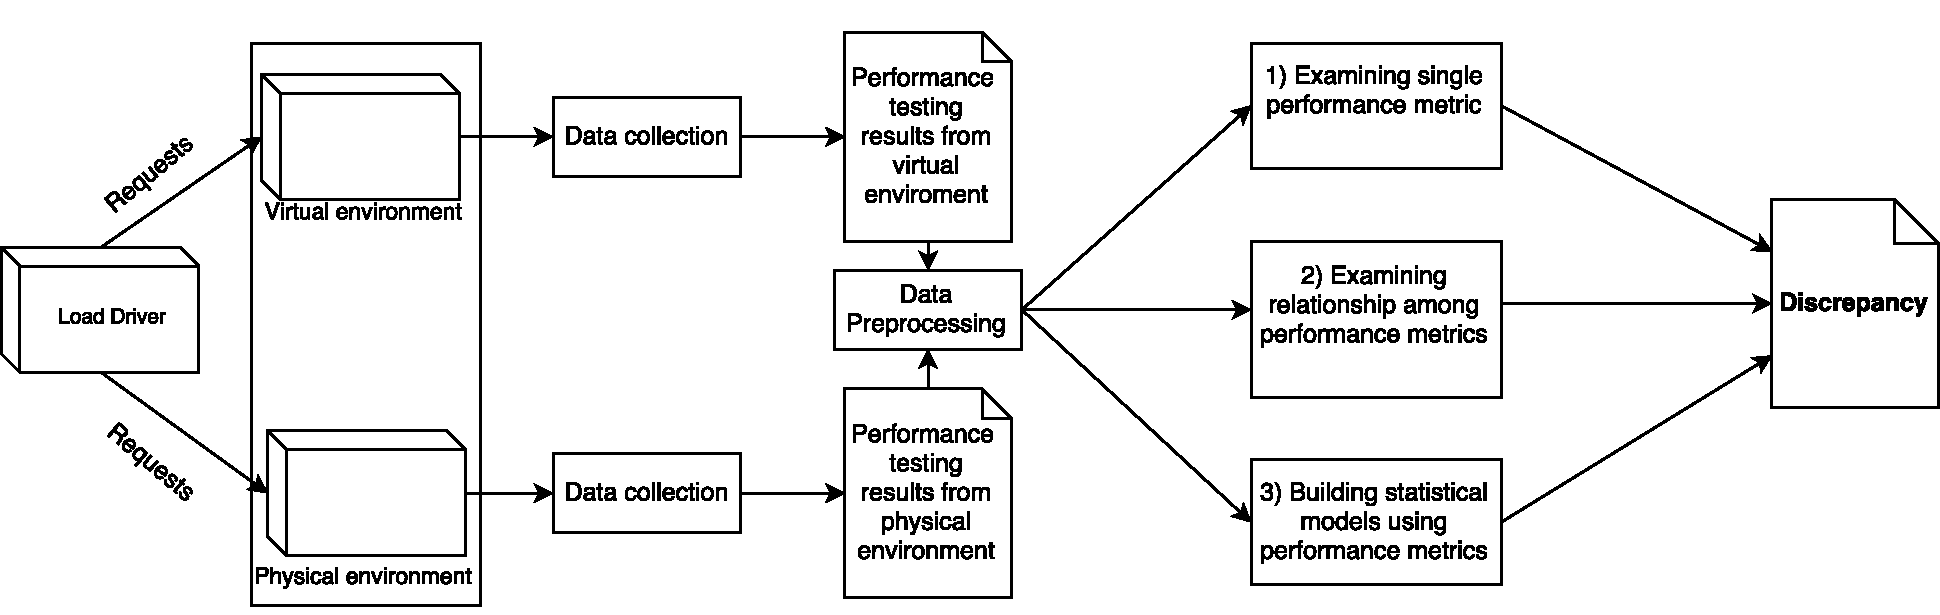
\includegraphics[width=.9\textwidth]{overview}
	\caption{An overview of our case study setup.}
	%\captionsetup{justification=centering}
	\label{fig:Approach}
\end{figure}

The goal of our case study is to evaluate the discrepancy between performance testing results from virtual and physical environments. We deploy our subject systems in two identical environments(physical and virtual). A load driver is used to exercise our subject systems. After the collection and processing of the performance metrics we analyze and draw conclusions based on: 1) individual performance metrics 2) relationship among performance metrics and 3) statistical models based on the performance metrics. An overview of our case study setup is shown in Figure~\ref{fig:Approach}.


\subsection{Subject Systems}
Dell DVD Store (DS2)~\cite{delldvd} is an online multi-tier e-commerce web application that is widely used in performance testing and prior performance engineering research~\cite{Shang:2015:ADP:2668930.2688052,Nguyen:2012:ADP:2188286.2188344, jackicsm2009}. We deploy DS2 (SLOC $>$ 3200) on an Apache (Version 3.0.0) web application server with MySQL 5.6 database server~\cite{mysql}. CloudStore~\cite{cloudstore}, our second subject system, is an open source application based on the TPC-W benchmark~\cite{tpcw}. CloudStore (SLOC $>$ 7600) is widely used to evaluate the performance of cloud computing infrastructure when hosting web-based software systems and is leveraged in prior research~\cite{tarekmsr16}. We deploy CloudStore on \textit{Apache Tomcat}~\cite{tomcat} (version 7.0.65) with MySQL 5.6 database server~\cite{mysql}.


\subsection{Environmental Setup}

The performance tests of the two subject systems are conducted on three machines in a lab environment. Each machine has an Intel i5 4690 Haswell Quad-Core 3.50 GHz CPU, with 8 GB of memory, 100GB SATA storage and connected to a local gigabyte ethernet. The first machine hosts the application servers (Apache and Tomcat). The second machine hosts the MySQL 5.6 database server. The load drivers were deployed on the third machine. We separate the load driver, the web/application server and the database server on different machines in order to mimic real world scenario and avoid interference among these processes. For example, isolating the web and database driver would ensure that the processor is not overused. The operating systems on the three machines are Windows 7. We disable all other processes and unrelated system services to minimize their performance impact. Since our goal is to compare performance metrics in virtual and physical environments, we setup the two different environments, which we detail next.


\noindent \textbf{Virtual environment.} We install one Virtual Box (version 5.0.16) and create only one virtual machine on one physical machine to avoid the interference between virtual machines. For each virtual machine, we allocate two cores and three gigabytes of memory, which is well below capacity to make sure we are topping out and pushing our configuration for unrealistic results. Virtual machines typically have an option of using disk pass-through\cite{whatisdiskpassthrough}. However, disk pass-through prevents the quickly deployment of an existing virtual machine image that’s designed for performance testing and start performance tests right away~\cite{diskpassthrough}. Hence, we opt not to enable disk pass-through since it is unlikely to be used in practice. The network of the virtual machine is set up based on NAT configuration\cite{NAT_config}. The network traffic of the workload was generated on dedicated load machine to keep our experiments as close to the real-world as possible.


\noindent \textbf{Physical environment.} We used the same hardware as the virtual environment to set up our physical environments. To make the physical environment similar to the virtual environment, we only enable two cores and three gigabytes of memory for each machine for the physical environment. 

\subsection{Performance tests}

DS2 is released with a dedicated load driver program that is designed to exercise DS2 for performance testing. We used the load driver to conduct performance testing on DS2. We used Apache JMeter~\cite{apachejmeter} to generate a workload to conduct the performance tests on CloudStore. For both subject systems, the workload of the performance tests is varied randomly and periodically in order to avoid bias from a consistent workload. The variation was identical across environments. The workload variation was introduced by the number of threads. A higher number of threads represent a higher number of users accessing the system. Each performance test is run after a 15 minute warming up period of the system and lasts for 9 hours. We chose to run the test 9 hours ensuring that our sample sizes have enough data points for our results to be statistically significant.
The nature of our performance tests was based on our related studies mentioned in section 2.2. To ensure the consistency between the performance tests, we restored the environments followed by a restart of the systems after every test.


\subsection{Data collection and preprocessing}

\noindent \textbf{Performance metrics.} We used \textit{PerfMon}~\cite{perfmon} to record the values of performance metrics. \textit{PerfMon} is a performance monitoring tool used to observe and record performance metrics such as CPU utilization, memory usage and disk IOs. We run \textit{PerfMon} on each of the application server or database server machine. We record all the available performance metrics that can be monitored on a single process by \emph{PerfMon}. In order to minimize influence by \textit{Perfmon}, we monitor only the performance of the two processes of the application server and database server on the two dedicated machines. We recorded the performance metrics with an interval of 10 seconds. In total, we recorded 44 performance metrics.

\noindent \textbf{System throughput.} We used the application server's access logs from Apache and Tomcat to calculate the throughput of the system by measuring the number of requests per minute. The two datasets were then concatenated and mapped against requests using their respective timestamps.

As an end user will consider a system as a whole. Therefore, we combine the performance datasets from our application and database server. In order to combine the two datasets of performance metrics and system throughput, and to minimize noise of the performance metric recording, we calculate the mean values of the performance metrics in every minute. Then, we combine the datasets of performance metrics and system throughput based on the time stamp on a per minute basis. A similar approach has been applied to address mining performance metrics challenges~\cite{foo2010mining}.



\section{Case Study Results}
\label{sec:results}

The goal of our study is to evaluate the discrepancy between performance testing results from virtual and physical environments, particularly considering the impact of discrepancy on the analysis of such results. We do not predict the applications' performance or throughput based on the amount of work done by the underlying architecture or the overhead induced by the virtual environment. Instead, our experiments are set in the context of analyzing performance testing data, based on the related work. Shown in Section~\ref{sec:related}, prior research and practitioners examines performance testing results in three types of approaches: 1) examining single performance metric, 2) examining the relationship among performance metrics and 3) building statistical models using performance metrics. Therefore, our experiments are designed to answer three research questions, where each questions corresponds to one approach above.



\subsection{Are the trend and distribution of an single performance metric similar across environments?}
\label{sec:individual}


\noindent \textbf{Motivation.}
\ian{make sure the wording: individual metrics => single metric}
The most intuitive approach of examining performance testing results is to examine every single performance metric. As shown in Section~\ref{sec:relatedindividual}, prior studies propose different approaches that typically compare the distribution or trend of each performance metric from different tests. Due to influences from testing environments, performance testing results are not expected to be identical in raw values. However, the shape of distribution and the trend of the metrics should not be similar. For example, if in one environment, we observe the Memory has increasing trend while the increasing trend is not seen in another environment, we observe a discrepancy. In addition, the distribution differences between two test results should not be statistically significant. Therefore, we use QQ plot and normalized KS tests to examine the differences in trends and shape of the distributions. 


\noindent \textbf{Approach.} 
After running and collecting the performance metrics, we compare every single performance metric between the virtual and physical environments. Since the performance tests are conducted in different environments, intuitively the scales of performance metrics are not the same. For example, the virtual environment may have higher CPU usage than the physical environment. Therefore, instead of comparing the values of each performance metric in both environments, we study whether the performance metric follows the same shape of the distribution and the same trend in virtual and physical environments. 

First, we plot a quantile-quantile plot (Q-Q plot)~\cite{qqplots} for every performance metric in two environments. A Q-Q plot is a plot of the quantiles of the first data set against the quantiles of the second data set. We also plot a 45-degree reference line on the Q-Q plots. If the performance metrics in both environments follow the same shape of distribution, the points on the Q-Q plots should fall approximately along this reference (i.e., 45-degree) line. A large departure from the reference line indicates that the performance metrics in the virtual and physical environments come from populations with different shapes of distributions, which can lead to a different set of conclusions. For example, the virtual environment has a CPU's utilization spike at a certain time, but the spike is absent in the physical environment. 

Second, to quantitatively measure the discrepancy, we perform a Kolmogorov-Smirnov test~\cite{kstest} between every performance metric in the virtual and physical environments. Since the scales of each performance metric in both environments are not the same, we first normalize the metrics based on their median values and their median absolute deviation: 
\begin{equation}
\label{equ:mad}
M_{normalized}=\frac{M-\tilde{M}}{MAD(M))}		
\end{equation}

where $M_{normalized}$ is the normalized value of the metric, $M$ is the original value of the metric, $\tilde{M}$ is the median value of the metric and $MAD(M)$ is the median absolute deviation of the metric~\cite{walker1929studies}. The Kolmogorov-Smirnov test gives a p-value as the test outcome. A p-value $\leq$ 0.05 means that the result is statistically significant, and we may reject the null hypothesis (i.e., two populations are from the same distribution). By rejecting the null hypothesis, we can accept the alternative hypothesis, which tells us the performance metrics in virtual and physical environments do not have the same distribution. We choose to use the Kolmogorov-Smirnov test since it does not have any assumption on the distribution of the metrics.

Finally, we calculate Spearman's rank correlation between every performance metric in the virtual environment and the corresponding performance metric in the physical environment, in order to assess whether the same performance metrics in two environments follow the same trend during the test. Intuitively, two sets of performance testing results without discrepancy should show similar trend, i.e., when memory keeps increasing in the physical environment (like memory leak), the memory should also increase in the virtual environment. We choose Spearman's rank correlation since it does not have any assumption on the distribution of the metrics. 

\noindent \textbf{Results.}
\textbf{Most performance metrics do not follow the same shape of distribution in virtual and physical environments.} Figure~\ref{fig:qqds2} and \ref{fig:qqcs} show the Q-Q plots by comparing the quantiles of performance metrics from virtual and physical environments. Due to the limited space, we only present Q-Q plot for CPU user time, IO data operations/sec and memory working set for both application sever and database server\footnote{The complete results are shared online at http://das.encs.concordia.ca/wp-content/uploads/2016/04/Arif\_results.zip}. The results show that the lines on the Q-Q plot are not close to the 45-degree reference line. By looking closely on the Q-Q plots we find that the patterns of each performance metric from different subject systems are different. For example, the web CPU user time for DS2 in the virtual environment shows higher values than in the physical environment at the median to high range of the distribution; while the Q-Q plot of CloudStore shows web CPU user time with higher values at the low range of the distribution. In addition, the lines of the Q-Q plots for database memory working set show completely different shapes in DS2 and in CloudStore. The results imply that the discrepancies between virtual and physical environments are present between the subject systems. The impact of the subject systems warrants its own study.

The majority of the performance metrics had statistically significantly different distributions (p-values lower than 0.05 in Kolmogorov-Smirnov tests). Only 13 and 12 metrics (out of 44 for each environment) have p-values higher than 0.05, for DS2 and CloudStore, respectively, showing statistically in-significant difference between the distribution in virtual and physical environments. By looking closely at such metrics, we find that these metrics either do not highly relate to the execution of the subject system (e.g., application server CPU privileged time in DS2), or highly relate to the workload. Since the workload between the two environments are similar, it is expected that the metrics related to the workload follow the same shape of distribution. For example, the I/O operations are highly related with the workload. The metrics related to I/O operations may show statistically in-significant differences between the distributions in the virtual and physical environments (e.g., application server I/O write operations per second in DS2). %\emad{should we list the metrics}


\textbf{Most performance metrics do not have the same trend in virtual and physical environments.} Table~\ref{tab:correlationrq1} shows the Spearman correlation coefficient and corresponding p-value between the selected performance metrics for which we shared the Q-Q plots. We find that for the application server memory working set in CloudStore and the database server memory working set in DS2, there exists strong (0.69) to moderate (0.46) correlation between the virtual and physical environments, respectively. By examining the metrics, we find that both metrics have an increasing trend that may be caused by a memory leak. Such increasing trend may be the cause of the moderate to strong correlation. Instead of showing the selected metrics as the Q-Q plots, Table~\ref{tab:correlationall} shows a summary of the spearman's rank correlation of all the performance metrics. Most of the correlations have an absolute value of 0 to 0.3 (low correlation), or the correlation is not statistically significant (p-val\textgreater0.05).

\textbf{Impact on the interpretation of examining single performance metric.} Practitioners often plot the trend of each important performance metrics, identify when the outliers exist or calculate the median or mean value of the metric to understand the performance of the system in general. However, based on our findings in this RQ, such analysis results may not be useful if they are from a virtual environment. For example, shown in Figure~\ref{fig:qqds2} and~\ref{fig:qqcs} many differences between the two distribution are in lower and higher ends of the plots, which corresponds to the high and low values of the metrics. Such values are often treated as outliers to be examined. However, if such outliers are due to the virtual environment rather than the system itself, the results may mislead. In addition, since the distribution of the metrics are statistically different, the mean and median value of the metrics may also mislead. 

\noindent\fbox{%
	\parbox{\textwidth}{%
		\textbf{Findings: }Performance metrics typically do not follow the same distribution in virtual and physical environments.\\ 
		\textbf{Actionable implications: }Practitioners cannot assume an straightforward overhead from the virtual environment nor compare single performance metric after applying a simple scaling factor to the metric.  
	}%
}


\begin{figure}[thb]
	\centering
	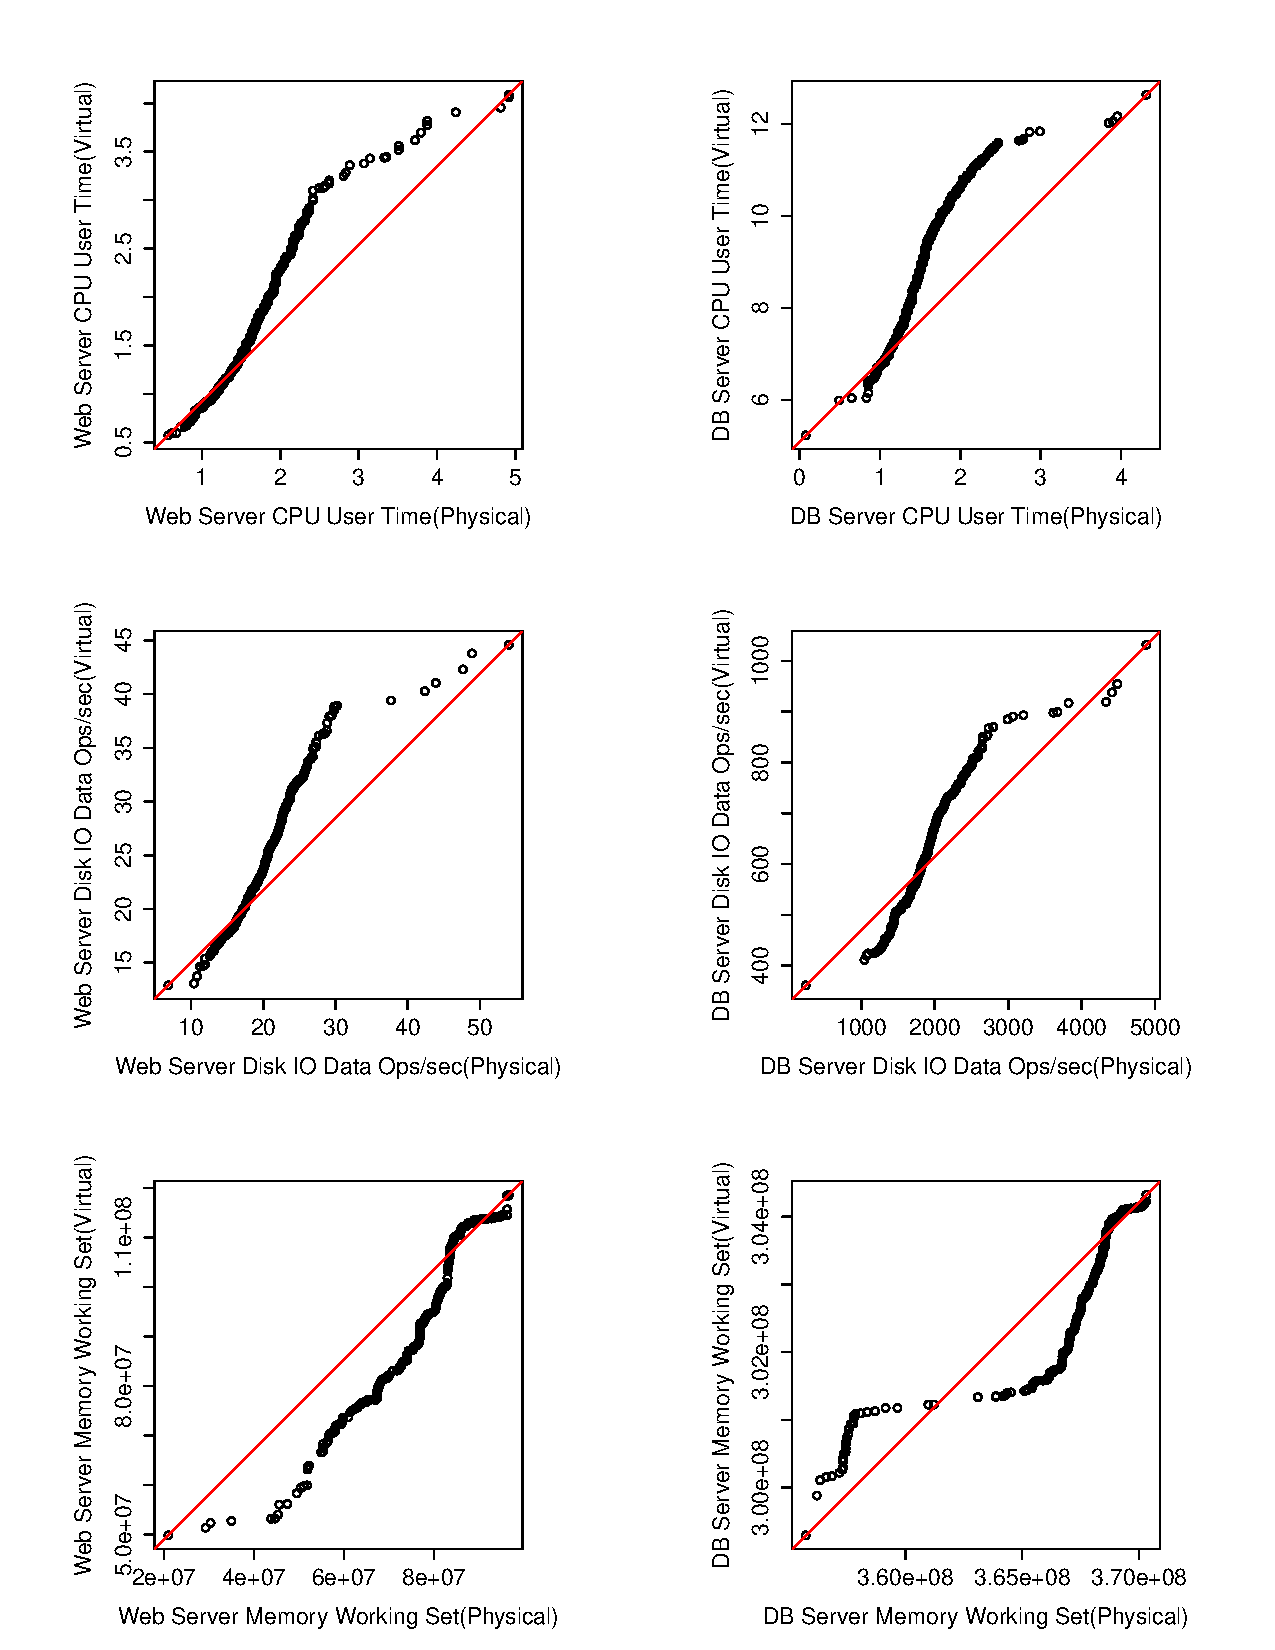
\includegraphics[width=0.9\columnwidth]{DS2_qq.pdf}
	\caption{Q-Q plots for DS2.}
	\label{fig:qqds2}
\end{figure}



\begin{figure}[thb]
	\centering
	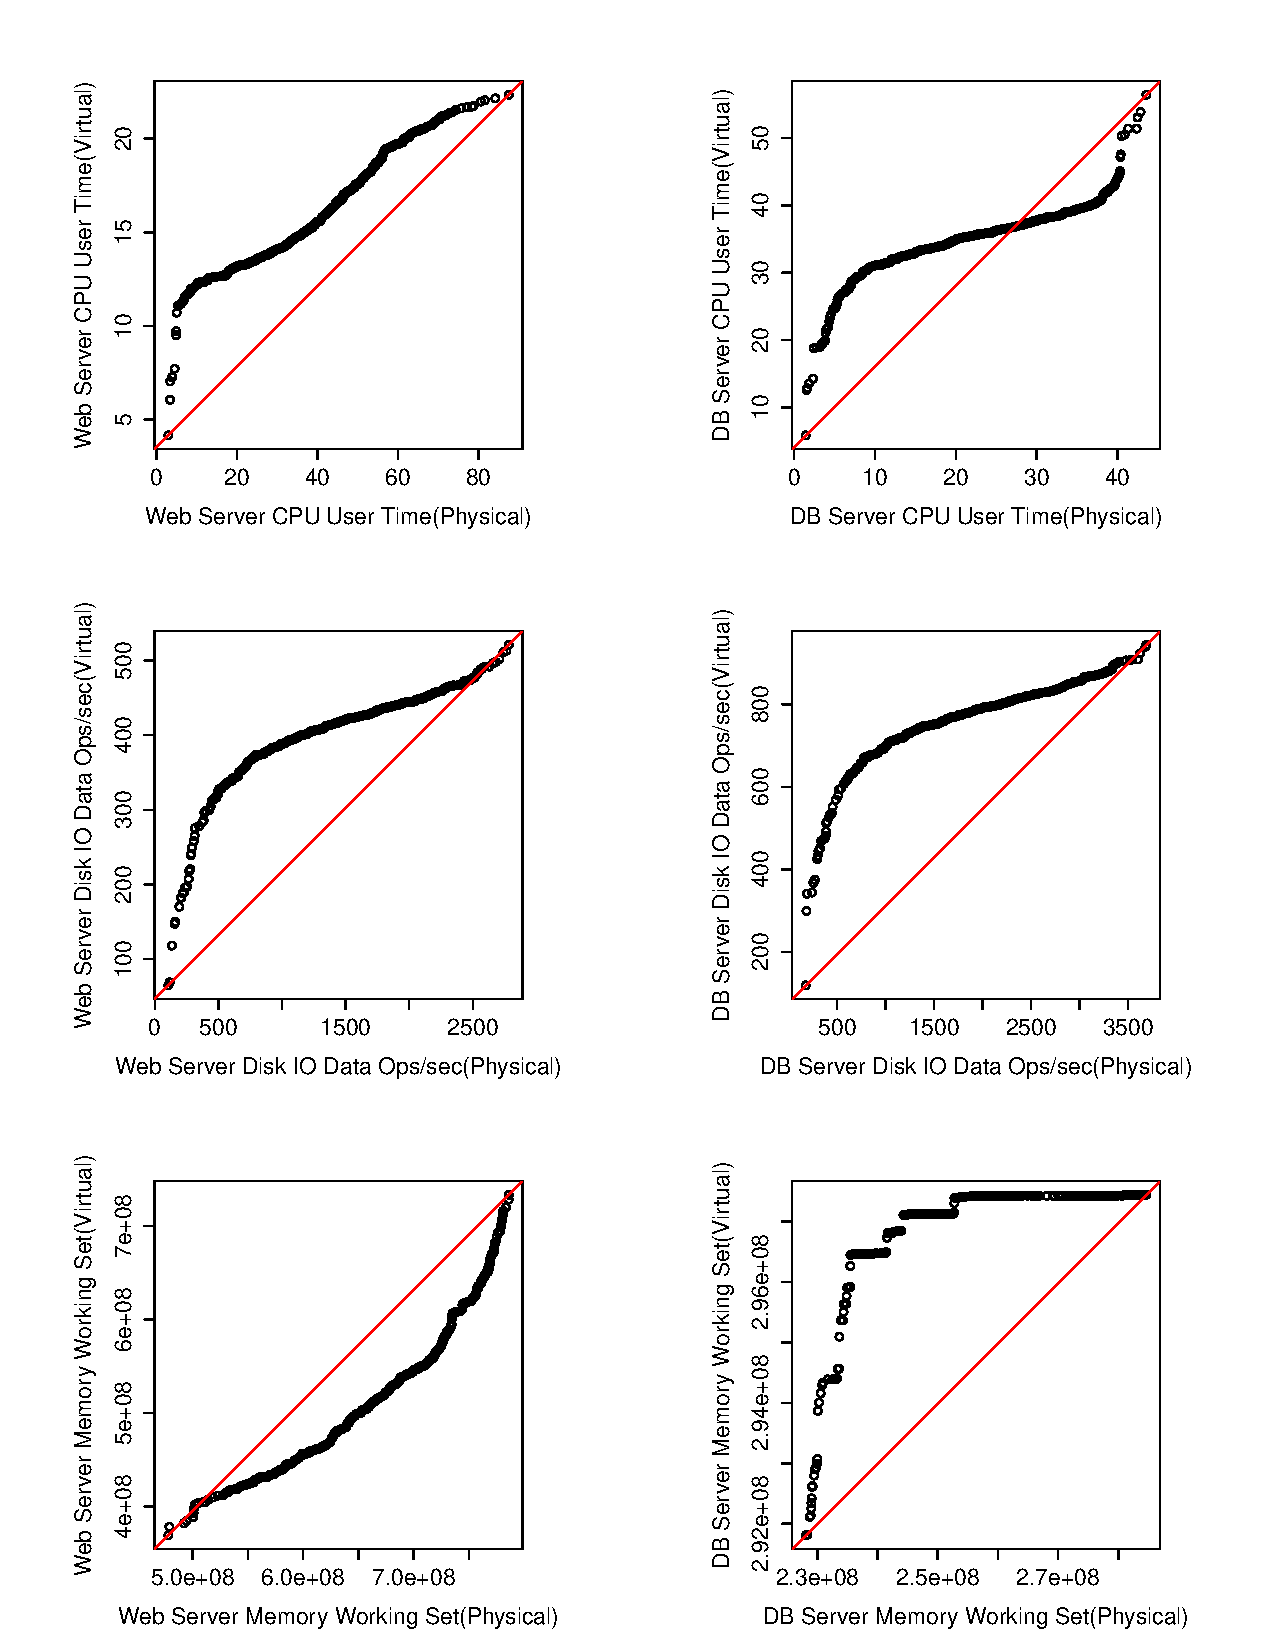
\includegraphics[width=0.9\columnwidth]{CS_qq.pdf}
	\caption{Q-Q plots for CloudStore.}
	\label{fig:qqcs}
\end{figure}



\begin{table}[thb]
	\centering
	\caption{Spearman's rank correlation coefficients and p-values of the highlighted performance metrics.}
	\label{tab:correlationrq1}
	\begin{tabular}{|c||c|c|c|c|}
		\hline
		\multirow{2}{*}{\textbf{Performance Metrics}} & \multicolumn{2}{c|}{\textbf{DS2}} & \multicolumn{2}{c|}{\textbf{CloudStore}} \\ \cline{2-5} 
		& \textbf{coef.} & \textbf{p-value} & \textbf{coef.} & \textbf{p-value} \\ %\hline
		\midrule 
		\midrule 
		Web Servers' User Times & 0.08 & 0.07 & -0.04 & 0.33 \\ \hline
		DB Servers User Times & -0.05 & 0.30 & 0.10 & 0.02 \\ \hline
		Web Servers' IO Data Ops/sec & 0.25 & 0.00 & 0.13 & 0.00 \\ \hline
		DB Servers' IO Data Ops/sec & -0.14 & 0.00 & 0.13 & 0.00 \\ \hline
		Web Servers' Memory Working Set & 0.22 & 0.00 & 0.69 & 0.00 \\ \hline
		DB Servers' Memory Working Set & 0.46 & 0.00 & -0.16 & 0.00 \\ \hline
	\end{tabular}
\end{table}

\begin{table}[tbh]
	\centering
	\caption{Summary of spearman's rank correlation p-values and absolute coefficients of all the performance metrics in DS2 and CloudStore. The numbers in the table are the number of metrics that fall into each category.}
	\label{tab:correlationall}
	\begin{threeparttable}
		
		\begin{tabular}{|c||c|c|c|c|c|}
			\hline
			\multirow{3}{*}{\textbf{System}} & \multirow{3}{*}{\textbf{p-value\textgreater0.05}} & \multicolumn{4}{c|}{\textbf{p-value\textless0.05}} \\ \cline{3-6} 
			&  & \textbf{0.0$\sim$0.3} & \textbf{0.3$\sim$0.5} & \textbf{0.5$\sim$0.7} & \textbf{0.7$\sim$1} \\ %\hline
			\midrule 
			\midrule 
			\textbf{DS2} & 8 & 28 & 4 & 0 & 1 \\ \hline
			\textbf{CloudStore} & 5 & 25 & 4 & 4 & 3 \\ \hline
		\end{tabular}%
		\begin{tablenotes}
			\item Three metrics are constant. Therefore, we do no calculate the correlation on those metrics.
		\end{tablenotes}
	\end{threeparttable}
	
\end{table}



\subsection{To what extend does the relationship between the performance metrics change across environments?}

\label{sec:relation}

\noindent \textbf{Motivation.}
The relationship between two performance counters may significantly change between two environments, which may be a hint of performance issues or system regressions. 
%We have used the following approach to examine the relationships between the performance metrics. 
As found by Cohen \emph{et al$.$}~\cite{cohen2004correlating}, combinations of performance metrics are significantly more predictive towards performance issues than single metric. A change in these combinations can reflect the discrepancy of performance and can help a practitioner identify the behavioral changes of a system between the two environments. For instance, in one release of the system, the CPU may be highly correlated with I/O while (e.g., when I/O is high, CPU is also high); while on a new release of the system, the correlation between CPU and I/O may become low. Such change to the correlation may expose a performance issue (e.g., the high CPU without I/O operation may be due to a performance bug). However, if there is a significant difference in correlations simply due to the platform being used, i.e., virtual vs. physical, then practitioners may need to be warned that a correlation discrepancy may be false. Therefore, we examine whether the relationship among performance metrics has a discrepancy between the virtual and physical environments. 


\noindent \textbf{Approach.} 
We calculate Spearman's rank correlation coefficients among all the metrics from each performance test in each environment. Then we study whether such correlation coefficients are different between the virtual and physical environments. 

First, we compare the changes in correlation between the performance metrics and the system throughput. For example, in one environment, the system throughput may be highly correlated with CPU; while in another environment, such correlation is low. In such a case, we consider there to be a discrepancy in the correlation coefficient between CPU and the system throughput. Second, for every pair of metrics, we calculate the absolute difference between the correlation in two environments. For example, if CPU and Memory have a correlation of $0.3$ in the virtual environment and $0.5$ in the physical environment, we report the absolute difference in correlation as $0.2$ ($|0.3-0.5|$). Since we have 44 metrics in total, we plot a heatmap in order to visualize the 1,936 absolute difference values between every pair of performance metrics. The lighter the color for each block in the heatmap, the larger the absolute difference in correlation between a pair of performance metrics. With the heatmap, we can quickly spot the metrics that have large discrepancy in correlation coefficients. 


\noindent \textbf{Results.}
\noindent \textbf{The correlation between system throughput and performance metrics changes between virtual and physical environments.} Tables~\ref{tab:top10ds2p} and~\ref{tab:top10csp} present the top ten metrics with the highest correlations to system throughput in the physical environment for DS2 and CloudStore, respectively. We chose system throughput to be our touchstone as it was kept identical between the environments.  We find that for these top ten metric sets, the difference in correlation coefficients in virtual and physical environments is up to \textbf{0.78} and the rank changes from \#9 to \#40 in DS2 and \#1 to \#10 in CloudStore.

\noindent \textbf{There exist differences in correlation among the performance metrics from virtual and physical environments.} Figures~\ref{fig:heatmap} and~\ref{fig:heatmap_cs} present the heatmap showing the changes in correlation coefficient among the performance metrics from virtual and physical environments. By looking at the heatmap, we find hotspots (with lighter color), which have larger correlation differences. For the sake of brevity, we do not show all the metric names in our heatmaps. Instead, we enlarge the heatmap by showing one of the hotspots for each subject system in Figures~\ref{fig:heatmap} and~\ref{fig:heatmap_cs}. We find that the hotspots correspond to the changes in correlation among I/O related metrics. Prior research on virtual machines has similar findings about I/O overheads in virtual machines~\cite{menon2005diagnosing,kraft2011io}. In such a situation, when practitioners observe that the relationship between I/O metrics and other metrics change, the change may not indicate a performance regression, but rather the change may be due to the use of a virtual environment.

\textbf{Impact on the interpretation of examining correlations between performance metric.} When a system is reported to have performance issues, correlations between metrics are often used in practice, as describe in the motivation of this RQ. However, since such correlation can be inconsistent in virtual and physical environment, existing knowledge of assumptions of correlation may not exist or new correlation may emerge, due to the use of virtual environment. For example, practitioners of a database-centric system may have the knowledge that I/O traffic is correlated with CPU and system throughput. Examining these three metrics together can help diagnosing performance issues, while if exist no such correlation in the virtual environment, these three metrics together may not be as useful in performance issue diagnosis.

\noindent\fbox{%
	\parbox{\textwidth}{%
		\textbf{Findings: }The correlations between performance metrics and system load may change considerably between virtual and physical environments. The correlation among performance metrics may also change considerably between virtual and physical environments. The correlations that are related with I/O metrics have the largest discrepancy.\\
		\textbf{Actionable implications: }Practitioners should always verify whether the inconsistency of correlations between performance metrics (especially I/O metrics) are due to virtual environments.
	}%
}


\begin{figure}[tbh]
	\centering
	{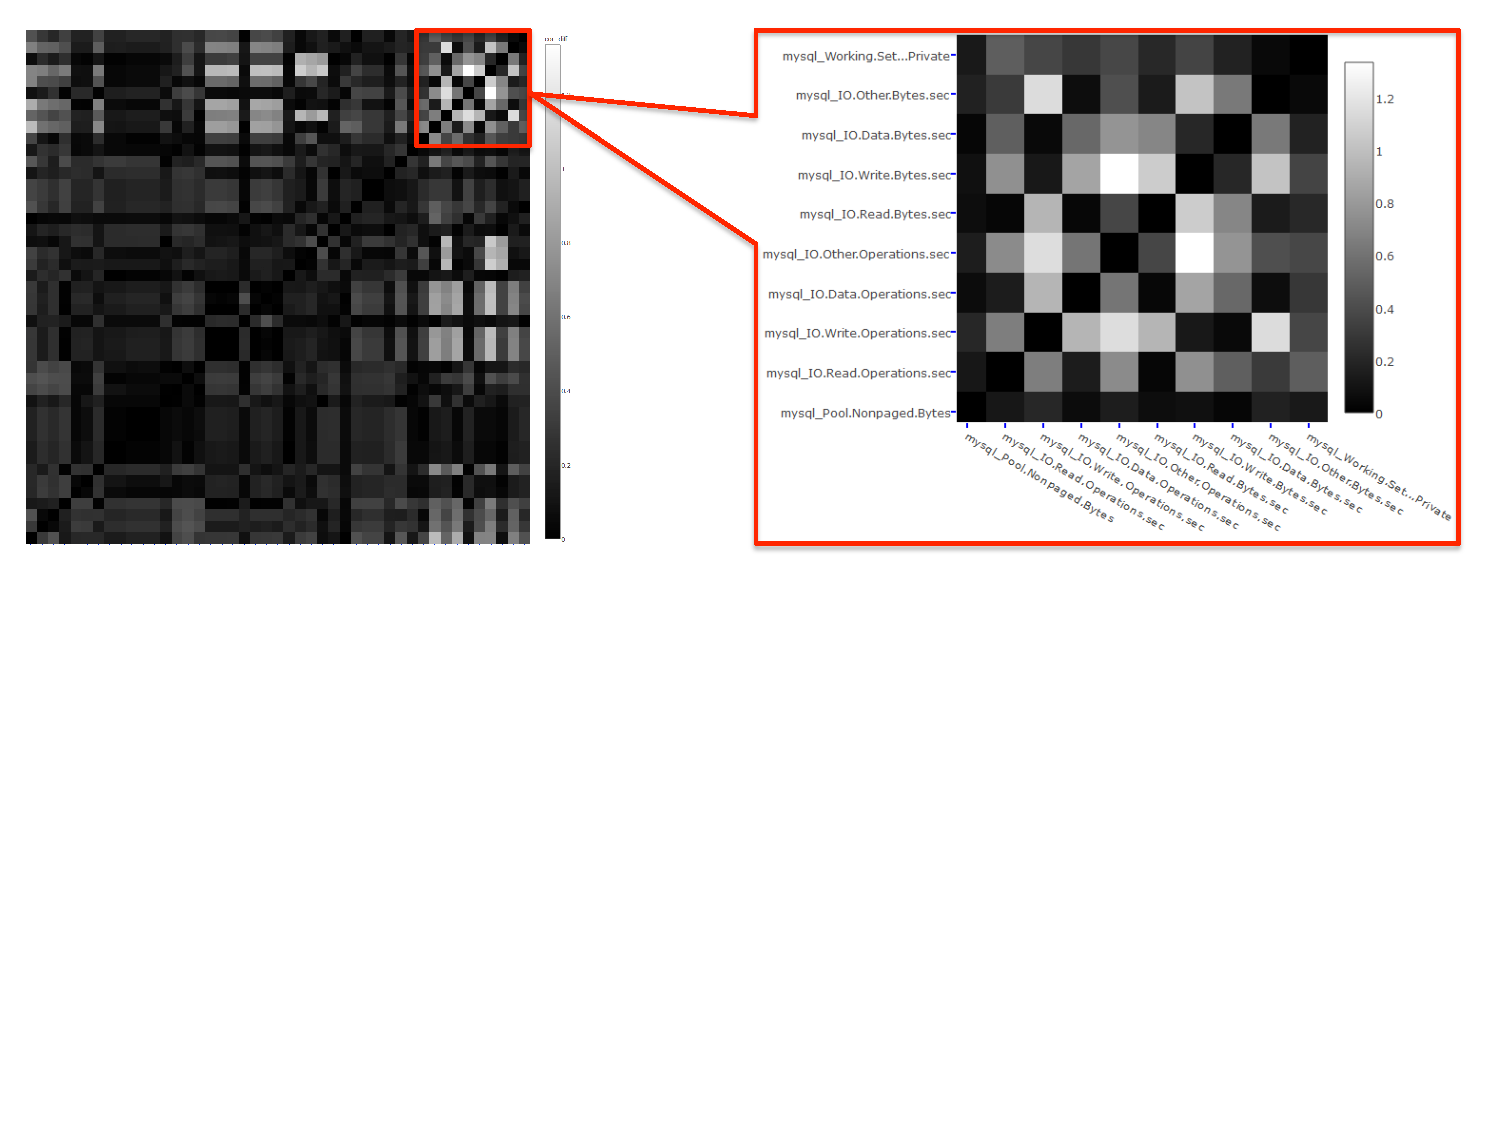
\includegraphics[width=1.0\textwidth]{heatmap_DS2}}
	\caption{Heatmap of correlation changes for DS2.}
	%\captionsetup{justification=centering}
	\label{fig:heatmap}
\end{figure}


\begin{figure}[tbh]
	\centering
	{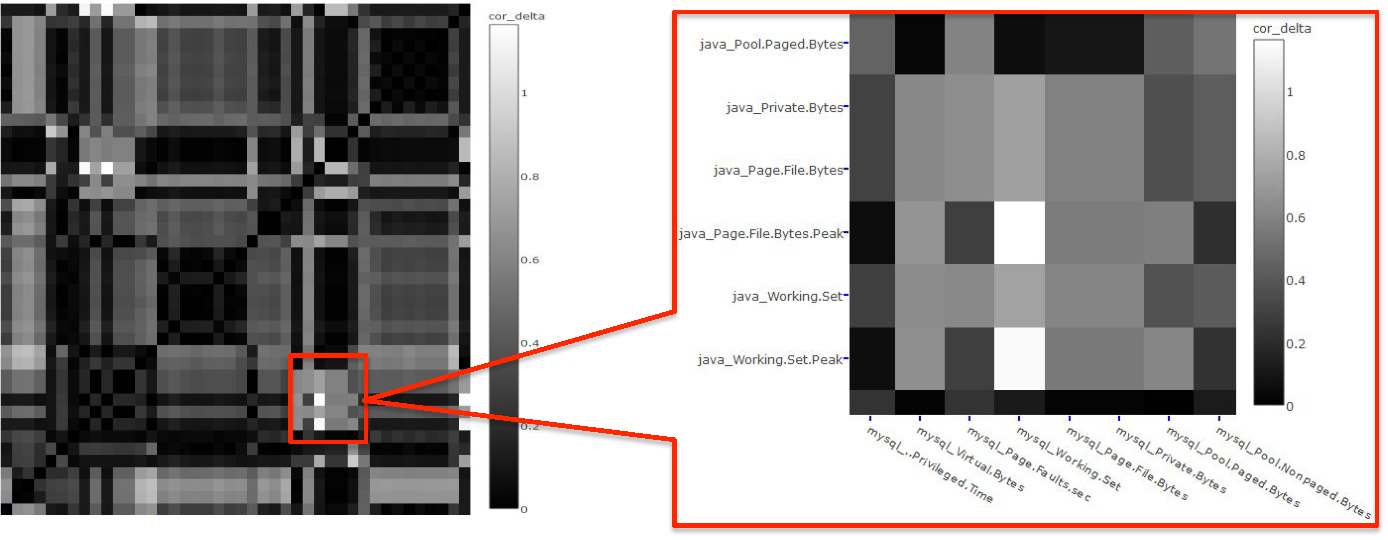
\includegraphics[width=1.0\textwidth]{heatmap_CS}}
	\caption{Heatmap of correlation changes for CloudStore.}
	%\captionsetup{justification=centering}
	\label{fig:heatmap_cs}
\end{figure}





\begin{table}[tbh]
	\centering
	\caption{Top ten metrics with highest correlation coefficient to system throughput in the physical environment for DS2. }
	\label{tab:top10ds2p}
	\begin{threeparttable}
		
		\begin{tabular}{|c||c|c|c|c|}
			\hline
			\textbf{Rank} & \textbf{Performance } & \textbf{Coef. } & \textbf{Coef. } & \textbf{Rank in} \\ %\hline
			& \textbf{ Metrics} & \textbf{PE} & \textbf{VE} & \textbf{VE} \\ %\hline
			\midrule
			\midrule
			1 & Web IO Other Ops/sec & 0.91 & 0.62 & 10 \\ \hline
			2 & Web IO Other Bytes/sec & 0.91 & 0.62 & 12 \\ \hline
			3 & Web IO Write Ops/sec & 0.91 & 0.63 & 9 \\ \hline
			4 & Web IO Data Ops/sec & 0.91 & 0.63 & 8 \\ \hline
			5 & Web IO Write Bytes/sec & 0.90 & 0.62 & 11 \\ \hline
			6 & Web IO Data Bytes/sec & 0.90 & 0.61 & 13 \\ \hline
			7 & DB IO Other Ops/sec & 0.84 & 0.75 & 3 \\ \hline
			8 & DB IO Data Ops/sec & 0.83 & 0.07 & 41 \\ \hline
			9 & DB IO Other Bytes/sec & 0.83 & 0.15 & 40 \\ \hline
			10 & DB IO Read Ops/sec & 0.82 & 0.15 & 39 \\ \hline
		\end{tabular}%
		\begin{tablenotes}
			\item PE in the table is short for physical environment; while VE is short for virtual environment.
		\end{tablenotes}
	\end{threeparttable}
	
	
\end{table}

\begin{table}[tbh]
	\centering
	\caption{Top ten metrics with highest correlation coefficient to system throughput in the physical environment for CloudStore}
	\label{tab:top10csp}
	\begin{threeparttable}
		
		\begin{tabular}{|c||c|c|c|c|}
			\hline
			\textbf{Rank} & \textbf{Performance } & \textbf{Coef. } & \textbf{Coef. } & \textbf{Rank in} \\ %\hline
			& \textbf{ Metrics} & \textbf{PE} & \textbf{VE} & \textbf{VE} \\ %\hline
			\midrule
			\midrule
			1 & DB Server IO Other Bytes/sec & 0.98 & 0.73 & 10 \\ \hline
			2 & DB Server IO Read Ops/sec & 0.98 & 0.84 & 7 \\ \hline
			3 & DB Server IO Read Bytes/sec & 0.98 & 0.93 & 5 \\ \hline
			4 & DB Server IO Write Ops/sec & 0.98 & 0.97 & 2 \\ \hline
			5 & DB Server IO Data Ops/sec & 0.98 & 0.92 & 6 \\ \hline
			6 & DB Server IO Data Bytes/sec & 0.98 & 0.96 & 4 \\ \hline
			7 & DB Server IO Write Bytes/sec & 0.98 & 0.96 & 3 \\ \hline
			8 & Web Server IO Other Bytes/sec & 0.98 & 0.68 & 16 \\ \hline
			9 & DB Server IO Other Ops/sec & 0.98 & 0.98 & 1 \\ \hline
			10 & Web Server IO Other Ops/sec & 0.98 & 0.70 & 14 \\ \hline
		\end{tabular}%
		\begin{tablenotes}
			\item PE in the table is short for physical environment; while VE is short for virtual environment.
		\end{tablenotes}
	\end{threeparttable}
	
	
\end{table}


\subsection{Can statistical performance models be applied across virtual and physical environments?}
\label{sec:model}
 

\noindent \textbf{Motivation.}
As discussed in the last research question (see Section~\ref{sec:relation}), the relationship among performance metrics is critical for examining performance testing results (see Section~\ref{sec:relatedrelation}). However, thus far we have only examined the relationships between two performance metrics. In order to capture the relationship among a large number of performance metrics, more complex modeling techniques are needed. Hence, we use statistical modeling techniques to examine the relationship among a set of performance metrics~\cite{xiong2013vperfguard,cohen2004correlating}. Moreover, some performance metrics do not have any impact with system performance, which are still examined. For example, for a software system that is CPU intensive, I/O operations may be irrelevant. Such performance metrics may expose large discrepancies between virtual and physical environments while not contributing to the examination of performance testing results. It is necessary to remove such performance metrics that are not contributing or impacting the results of the performance analysis. To address the above issues, modeling techniques are proposed to examine performance testing results (see Section~\ref{sec:relatedmodel}). In this step, we examine whether the modeling among performance metrics can apply across virtual and physical environments and whether we can minimize such discrepancy between performance models.


\noindent \textbf{Approach. }

%\emad{we should really add a reason as to why we are doing this}
We follow a model building approach that is similar to the approach from prior research~\cite{Shang:2015:ADP:2668930.2688052,Cohen:2005:CIC:1095810.1095821,xiong2013vperfguard}. We first build statistical models using performance metrics from one environment, then we test the accuracy of our performance model with the metric values from the same environment and also from a different environment. For example, if the model was built in a physical environment it was tested in both, physical and virtual environment.

\subsubsection{B-1: Reducing counters}

Mathematically, performance metrics that show little or no variation do not contribute to the statistical models hence we first remove performance metrics that have constant values in the test results. We then perform a correlation analysis on the performance metrics to remove multicollinearity based on statistical analysis~\cite{cor_R}. We used the Spearman's rank correlation coefficient among all performance metrics from one environment. We find the pair of performance metrics that have a correlation higher than 0.75~\cite{Syer2016}. From these two performance metrics, we remove the metric that has a higher average correlation with all other metrics. We repeat this step until there exists no correlation higher than 0.75.

We then perform redundancy analysis on the performance metrics. The redundancy analysis would consider a performance metric redundant if it can be predicted from a combination of other metrics~\cite{harrell2001regression}. We use each performance metric as a dependent variable and use the rest of the metrics as independent variables to build a regression model. We calculate the $R^2$ of each model. $R^2$, or the coefficient of multicollinearity, is used to analyze how a change in one of the variables (e.g. predictor) can be explained by the change in the second variable (e.g. response) \cite{rsquare}. We consider multicollinearity to be present if more than one predictor variable can explain the change in the response variable. If the $R^2$ is larger than a threshold (0.9)\cite{Syer2016}, the current dependent variable (i.e., performance metric) is considered redundant. We then remove the performance metric with the highest $R^2$ and repeat the process until no performance metric can be predicted with $R^2$ higher than the threshold. For example, if CPU can be linearly modeled by the rest of the performance metrics with $R^2\textgreater0.9$, we remove the metric for CPU.

Not all the metrics in the model are statistically significant. Therefore in this step, we only keep the metrics that have a statistically significant contribution to the model. We leverage the \textit{stepwise} function that adds the independent variables one by one to the model to exclude any metrics that are not contributing to the model~\cite{RInAction}. 

\subsubsection{B-2: Building statistical models}

In the second step, we build a linear regression model~\cite{freedman2009statistical} using the performance metrics that are left after the reduction and removal of statistically insignificant metrics in the previous step as independent variables and use the system throughput as our dependent variable. We chose the linear regression model over other models because of its uncomplicated explanation. Hence, it is easier to interpret the discrepancy that is illustrated by the model. Similar models have been built in prior research~\cite{Cohen:2005:CIC:1095810.1095821,xiong2013vperfguard,Shang:2015:ADP:2668930.2688052}.

%\subsubsection{B-3: Finalizing statistical models}
After removing all the insignificant metrics, we have all the metrics that significantly contribute to the model. We use these metrics as independent variables to build the final model.

\subsubsection{V-1: Validating model fit}

Before we validate the model with internal and external data, we first examine how good the model fit is. If the model has a poor fit to the data, then our findings from the model may be biased by the noise from the poor model quality. We calculate the $R^2$ of each model to measure fit. If the model perfectly fits the data, the $R^2$ of the model is 1, while a zero $R^2$ value indicates that the model does not explain the variability of the response data. We also would like to estimate the impact that each independent variable has on the model fit. We follow a ``drop one'' approach~\cite{Chambers1990}, which measures the impact of an independent variable on a model by measuring the difference in the performance of models built using: (1) all independent variables (the full model), and (2) all independent variables except for the one under test (the dropped model). A Wald statistic is reported by comparing the performance of these two models ~\cite{harrell2001regression}. A larger Wald statistic indicates that an independent variable has a larger impact on the model's performance, i.e., model fit. A similar approach has been leveraged by prior research in~\cite{mcintosh2015emse}. We then rank the independent variables by their impact on model fit. 


\subsubsection{V-2: Internal validation}

We validate our models with the performance testing data that is from the same environment. We leverage a standard 10-fold cross validation process, which starts by partitioning the performance data to 10 partitions. We take one partition (fold) at a time as the test set, and train on the remaining nine partitions~\cite{10foldcross,kohavi1995study}, similar to prior research~\cite{haroon}. For every data point in the testing data, we calculate the absolute percentage error. For example, for a data point with a throughput value of 100 requests per minute, if our predicted value is 110 requests per minute, the absolute percentage error is $0.1$ ($\frac{|110-100|}{100}$). After the ten-fold cross validation, we have a distribution of absolute percentage error (\textit{MAPE}) for all the data records.



\subsubsection{V-3: External validation}
To evaluate whether the model built using performance testing data in one environment (e.g., virtual environment) can apply to another environment (e.g., physical environment), we test the model using the data from the other environment.

Since the performance testing data is generated from different environments, directly applying the data on the model would intuitively generate large amounts of error. We adopt two approaches in order to normalize the data in different environments: (1) \textbf{Normalization by deviance.} The first approach we use is the same when we compare the distribution of each individual performance counter shown in Equation~\ref{equ:mad} from Section~\ref{sec:individual} by calculating the relative deviance of a metric value from its median value. (2) \textbf{Normalization by load.} The second approach that we adopt is an approach that is proposed by Nguyen \textit{et al.}~\cite{Nguyen:2012:ADP:2188286.2188344}. The approach uses the load of the system to normalize the performance metric values across different environments. As there are varying inputs for the performance tests that we carried out, normalization by load helps in normalizing the multi-modal distribution that might be because of the trivial tasks like background processes(bookkeeping).



To normalize our metrics, we first build a linear regression model with the one metric as an independent variable and the throughput of the system as the dependent variable. With the linear regression model in one environment, the metric values can be represented by the system throughput. Then we normalize the metric value by the linear regression from the other environment. The details of the metric transformation are shown as follows:

\begin{equation*}
throughput_{p}= \alpha_{p} \times M_{p} + \beta_{p}
\end{equation*}
\vspace{-0.4cm}
\begin{equation*}
throughput_{v}= \alpha_{v} \times M_{v} + \beta_{v}
\end{equation*}
\vspace{-0.4cm}
\begin{equation*}
M_{normalized} = \frac{(\alpha_{v} \times M_{v})+\beta_{v}-\beta_{p}}{\alpha_{p}}
\end{equation*}
where $throughput_{p}$ and $throughput_{v}$ are the system throughput in the physical and virtual environment, respectively. $M_{p}$ and $M_{v}$ are the performance metrics from both environments, while $M_{normalized}$ is the metric after normalization. $\alpha$ and $\beta$ are the coefficient and intercept values for the linear regression models. After normalization, we calculate the absolute percentage error for every data record in the testing data.




\subsubsection{Identifying model discrepancy}
In order to identify the discrepancy between the models built using data from the virtual and physical environments, we compare the two distributions of absolute percentage error based on our internal and external validation. If the two distributions are significantly different (e.g., the absolute percentage error from internal validation is much lower than that from external validation), the two models are considered to have a discrepancy. To be more concrete, in total for each subject system, we ended up with four distributions of absolute percentage error: 1) modeling using the virtual environment and testing internally (on data from the virtual environment), 2) modeling using the virtual environment and testing externally (on data from the physical environment), 3) modeling using the physical environment and testing internally (on data from the physical environment), 4) modeling using the physical environment and testing externally (on data from the virtual environment). We compare distributions 1) and 2) and we compare distributions 3) and 4). Since normalization based on deviance will change the metrics values to be negative when the metric value is lower than median, such negative values cannot be used to calculate absolute percentage error. We perform a min-max normalization on the metric values before calculating the absolute percentage error. In addition, if the observed throughput value after normalization is zero (when the observed throughput value is the minimum value of both the observed and predicted throughput values), we cannot calculate the absolute percentage error for that particular data record. Therefore, we remove the data record if the throughput value after normalization is zero. In our case study, we only removed one data record when performing external validation with the model built in the physical environment. 


\noindent \textbf{Results.}

\noindent \textbf{The statistically significant performance metrics leveraged by the models in virtual and physical environments are not the same.} Tables~\ref{tab:modelsummaryds2} and \ref{tab:modelsummarycs} show the summary of the statistical models built for the virtual and physical environments for the two subject systems. We find that all the models have a good fit (66.9\% to 94.6\% $R^2$ values). However, some statistically significant independent variables in one model do not appear in the other model. For example, Web Server Virtual Bytes ranks \#4 for the model built from the physical environment data of CloudStore, while the metric is not significant in the model built from the virtual environment data. In fact, none of the significant variables in the model built from the virtual environment are related to the application server's memory (see Table~\ref{tab:modelsummarycs}). We do observe some performance metrics that are significant in both models even with the same ranking. For example, Web Server IO Other Bytes/sec is the \#1 significant metric for both models built from the virtual and physical environment data of DS2 (see Table~\ref{tab:modelsummaryds2}). 

\noindent \textbf{The prediction error illustrates discrepancies between models built in virtual and physical environments.} Although the significant independent variables in the models built by the performance testing results in the virtual and physical environments are different, the model may have similar prediction results due to correlations between metrics. However, we find that the external prediction errors are higher than internal prediction errors for all four models from the virtual and physical environments for the two subject systems. In particular, Table~\ref{tab:errors} shows the prediction errors using normalization based on load is always higher than that of the internal validation. For example, the median absolute percentage error for CloudStore using normalization by load is 632\% and 483\% for the models built in the physical environment and virtual environment, respectively; while the median absolute percentage error in internal validation is only 2\% and 10\% for the models built in the physical and virtual environments, respectively. However, in some cases, the normalization by deviance can produce low absolute percentage error in external validation. For example, the median absolute percentage error for CloudStore can be reduced to 9\% using normalization by deviance. 

One possible reason is that the normalization based on load performs better, even though it is shown to be effective in prior research~\cite{Nguyen:2012:ADP:2188286.2188344}, assumes a linear relationship between the performance metric and the system load. However, such an assumption may not be true in some performance testing results. For example, Table~\ref{tab:top10ds2p} shows that some I/O related metrics do have low correlation with the system load in virtual environments. On the other hand, the normalization based on deviance shows much lower prediction error. We think the reason is that the virtual environments may introduce metric values with high variance. Normalizing based on the deviance controls such variance, leading to lower prediction errors.



\begin{table}[tbh]
	\centering
	\caption{Summary of statistical models built for DS2. The metrics listed in the table are the significant independent variables.}
	\label{tab:modelsummaryds2}
	\resizebox{\columnwidth}{!}{%
		\begin{tabular}{|c||c|c|}
			\hline
			\textbf{Environment} & \textbf{Physical} & \textbf{Virtual} \\ %\hline
			\midrule
			\midrule
			\textbf{1} & Web Server IO Other Bytes/sec & Web Server IO Other Bytes/sec \\ \hline 
			\textbf{2} & Web Server Page Faults/sec & DB server Working Set - Peak \\ \hline
			\textbf{3} & DB Server Page Faults/sec & Web Server Virtual Bytes \\  \hline
			\textbf{4} & DB Server IO Write Bytes/sec & Web Server Page Faults/sec \\ \hline
			\textbf{5} & Web Server IO Read Bytes/sec & DB Server Page Faults/sec \\ \hline
			\textbf{6} & DB Server User Time & DB Server IO Data Ops/sec \\ \hline
			\textbf{7} & DB Server Pool Paged Bytes & -  \\ \hline
			\textbf{8} & DB Server Privileged Time &  - \\ \hline
			\midrule
			\textbf{$R^2$}  & 94.6\% & 66.90\% \\ \hline
			%			\textbf{MAPE} & 4.00\% & 10.52\% \\ \hline
		\end{tabular}%
	}
\end{table}


\begin{table}[tbh]
	\centering
	\caption{Summary of statistical models built for CloudStore. The metrics listed in the table are the significant independent variables.}
	\label{tab:modelsummarycs}
	\resizebox{\columnwidth}{!}{%
		\begin{tabular}{|c||c|c|}
			\hline
			\textbf{Environment} & \textbf{Physical} & \textbf{Virtual} \\ %\hline
			\midrule
			\midrule
			\textbf{1} & Web Server Privileged Time & Web Server IO Write Ops/sec \\ \hline
			\textbf{2} & DB Server Privileged Time & DB Server IO Read Ops/sec \\ \hline
			\textbf{3} & Web Server Page Faults/sec &  Web Server Privileged Time \\ \hline
			\textbf{4} & Web Server Virtual Bytes & DB Server Privileged Time \\ \hline
			\textbf{5} & Web Server Page File Bytes Peak &  DB Server IO Other Bytes/sec \\ \hline
			\textbf{6} & DB Server Pool Nonpaged Bytes & DB Server Pool Nonpaged Bytes \\ \hline
			\textbf{7} & DB Server Page Faults/sec & -  \\ \hline
			\textbf{8} & DB Server Working Set & - \\ %\hline
			\midrule
			\textbf{$R^2$} & 85.30\% & 90.20\% \\ \hline
			%		\textbf{MAPE} & 15.63\% & 3.65\% \\ \hline
		\end{tabular}%
	}
\end{table}
\begin{table}[tbh]
	\centering
	\caption{Internal and external prediction errors for both subject systems.}
	\label{tab:errors}
	\resizebox{\textwidth}{!}{%
		\begin{tabular}{|c||c|c|c|c|c|c|c|c|c|}
			\hline
			\multicolumn{9}{|c|}{\textbf{DS2}} \\ \hline
			\textbf{Model Built} & \multicolumn{2}{c|}{\textbf{Validation}} & \textbf{Min.} & \textbf{1st Quart.} & \textbf{Median} & \textbf{Mean} & \textbf{3rd Quart.} & \textbf{Max}\\ %\hline
			\midrule
			\midrule
			\multirow{3}{*}{\textbf{Physical}} & \multicolumn{2}{c|}{\textbf{Internal Validation}} & 0.00 & 0.01 & 0.02 & 0.03 & 0.05 & 0.30 \\ \cline{2-9} 
			& \multirow{2}{*}{\textbf{External Validation}} & \textbf{Normalization by Deviance} & 0.00 & 0.08 & 0.25 & 0.36 & 0.49 & 13.65 \\ \cline{3-9} 
			&  & \textbf{Normalization by Load} & 0.00 & 0.34 & 0.44 & 0.48 & 0.56 & 1.56  \\ \hline
			\multirow{3}{*}{\textbf{Virtual}} & \multicolumn{2}{c|}{\textbf{Internal Validation}} & 0.00 & 0.04 & 0.09 & 0.11 & 0.15 & 0.54 \\ \cline{2-9} 
			& \multirow{2}{*}{\textbf{External Validation}} & \textbf{Normalization by Deviance} & 0.00 & 0.09 & 0.20 & 0.27 & 0.34 & 2.82  \\ \cline{3-9} 
			&  & \textbf{Normalization by Load} & 0.00 & 0.06 & 0.13 & 0.17 & 0.23 & 0.92 \\ \hline
		\end{tabular}%
	}

	
	\vspace{2ex}
	
	\centering
	\resizebox{\textwidth}{!}{%
		\begin{tabular}{|c||c|c|c|c|c|c|c|c|}
			\hline
			\multicolumn{9}{|c|}{\textbf{CloudStore}} \\ \hline
			\textbf{Model Built} & \multicolumn{2}{c|}{\textbf{Validation}} & \textbf{Min.} & \textbf{1st Quart.} & \textbf{Median} & \textbf{Mean} & \textbf{3rd Quart.} & \textbf{Max}\\ \midrule
			\midrule
			\multirow{3}{*}{\textbf{Physical}} & \multicolumn{2}{c|}{\textbf{Internal Validation}} & 0.00 & 0..05 & 0.10 & 0.16 & 0.18 & 2.68\\ \cline{2-9} 
			& \multirow{2}{*}{\textbf{External Validation}} & \textbf{Normalization by Deviance} & 0.00 & 0.04 & 0.09 & 0.17 & 0.17 & 2.29  \\ \cline{3-9} 
			&  & \textbf{Normalization by Load} & 2.90 & 5.14 & 6.32 & 7.75 & 8.08 & 51.33 \\ \hline
			\multirow{3}{*}{\textbf{Virtual}} & \multicolumn{2}{c|}{\textbf{Internal Validation}} & 0.00 & 0.01 & 0.03 & 0.04 & 0.05 & 0.50  \\ \cline{2-9} 
			& \multirow{2}{*}{\textbf{External Validation}} & \textbf{Normalization by Deviance} & 0.00 & 0.03 & 0.07 & 0.11 & 0.13 & 1.00  \\ \cline{3-9} 
			&  & \textbf{Normalization by Load} & 4.07 & 4.64 & 4.83 & 5.13 & 5.10 & 33.36  \\ \hline
		\end{tabular}%
	}
	\vspace{-0.3cm}
\end{table}


\textbf{Impact on the interpretation of examining statistical performance models.} Statistical performance models are often used to interpret relationships among many system performance metrics. For example, what are the significant metrics that are associated with system load and what performance metrics are redundant. Since the statistical performance models have large discrepancy, even after applying normalization techniques that is proposed by prior research, we cannot directly use the performance models built in the virtual environment. Even though our results show that normalizing by deviance can reduce the discrepancy, practitioners should still be aware of it when examining the performance models.

\noindent\fbox{%
	\parbox{\textwidth}{%
		\textbf{Findings: }We find that the statistical models built by performance testing results in an environment cannot advocate for the other environment due to discrepancies present. Normalization technique for heterogeneous environments and workloads that is proposed by prior research may not work for virtual and physical environment.\\
		 \textbf{Actionable implications: }Normalizing the performance metrics by deviance may minimize such discrepancy and should be considered by practitioners before examining performance testing results. 
	}%
}
\section{Discussion}
\label{sec:discussion}

In the previous section, we find that there is a discrepancy between performance testing results from the virtual and physical environments. However, such discrepancy can also be due to other factors such 1) the instability of the virtual environments, 2) the virtual machine that we used or 3) the different hardware resources on the virtual environments. Therefore, in this section, we examine the impact of such factors to better understand our results. 


\subsection{Investigating the stability of virtual environments}

Thus far, we perform our case studies in one virtual environment and compare the performance metrics to the physical environment. However, the stability of the results obtained from the virtual environment need to be validated, in particular since VMs tend to be highly sensitive to the environment that they run in~\cite{leitner}.
 

In order to study whether the virtual environment is stable, we repeat the same performance tests, twice more, on the virtual environments for both subject systems. In total, we had results from three performance tests. We perform the data analysis in Section~\ref{sec:model} by building statistical models using performance metrics. %Table~\ref{tab:stabilityvm} shows the median absolute percentage error from building a model using one virtual environment and testing on another virtual environment. 
As the previously mentioned approach, we build a model based on one of the runs, serving as our training data for the model, and tested it on another run. In this case, we define external validation when a model is trained on a different run than it is tested on. We validate our model by predicting the throughput of a different run.  

Prediction error values (see section 4.3.5) closer to 0 indicate that our model was able to successfully explain the variation of the throughput of a different run. This also means that the external validation error closer to 1 or higher depicts instability of the environment. We find the external validation error to be 0.04 and 0.13 for CloudStore and DS2, respectively. The internal validation error is 0.03 and 0.09 for CloudStore and DS2, respectively. Such low error values show that the performance testing results from the virtual environments are rather stable. 

\subsection{Investigating the Impact of Specific Virtual Machine Software}

In all of our experiments, we used the Virtual Box software to setup our virtual environment. However, there exists a plethora of VM software (i.e., it can be argued that our chosen subject systems behave differently in another environment). The question that arises then is whether the choice of VM software impacts our findings. In order to address the aforementioned hypothesis, we set up another virtual environment using VMWare (version 12) with the same allocated computing resources as when we set up Virtual Box.

To investigate this phenomenon, we repeat the performance tests for both subject systems. We train statistical models on the performance testing results from VMWare and test on the results from both the original virtual environment data (Virtual Box) and the results from the physical environments. We could not apply the normalization by deviance for the data from VMWare since some of the significant metrics in the model have a median absolute deviance of 0, making the normalized metric value to be infinite (see Equation~\ref{equ:mad}). We only apply the normalization by load. 

Table~\ref{tab:vmware} shows that the performance testing results from the two different virtual machine software is similar, as supported by the low percentage error when our model was tested on Virtual Box. In addition, the high error when predicting with physical environment agrees with the results when testing with the performance testing results from the Virtual Box (see Table~\ref{tab:errors}). Such results show that the discrepancy observed during our experiment also exits with the virtual environments that are set up with VMWare.

\begin{table}[tbh]
	\centering
	\caption{Median absolute percentage error from building a model using VMWare data.}
	\label{tab:vmware}
	\begin{tabular}{|c||c|c|}
		\hline
		\multirow{2}{*}{\textbf{Validation type}} & \multicolumn{2}{c|}{\textbf{Median absolute percentage error}} \\ \cline{2-3} 
		& \textbf{CloudStore} & \textbf{DS2} \\ %\hline
		\midrule
		\midrule
		External validation with Virtual Box results& 0.07&0.10\\ \hline
		External validation with physical normalization by load & 7.52& 1.63 \\ \hline
	\end{tabular}
\end{table}

\subsection{Investigating the Impact of Allocated Resources}

Another aspect that may impact our results is the resources allocated and the configuration of the virtual environment. We did not decrease the system resources as decreasing the resources may lead to crashes in the testing environment.

To investigate the impact of the allocated resources, we increase the computing resources allocated to the virtual environments by increasing the CPU to be 3 cores and increasing the memory to be 5GB. We cannot allocate more resource to the virtual environment since we need to keep resources for the hosting OS. We train statistical models on the new performance testing results and tested it on the performance testing results from the physical environment. 

Similar to the results shown in Table~\ref{tab:errors}, the prediction error is high when we normalize by the load as per Equation~\ref{equ:mad} (1.57 for DS2 and 1.25 for CloudStore), while normalizing based on deviance can significantly reduce the error (0.09 for DS2 and 0.07 for CloudStore). We conclude that our findings still hold when the allocated resources are changed and this change has minimal impact on the results of our case studies.


	
\section{Threats to Validity}
\label{sec:threats}


\subsection{External validity.}
We chose two subject systems, CloudStore and DS2 for our study and two virtual machine software, VirtualBox and VMware. The two subject systems have years of history and prior performance engineering research has studied both systems~\cite{jackicsm2009,Nguyen:2012:ADP:2188286.2188344,tarekmsr16}. The virtual machine software that we used is widely used in practice. Nevertheless more case studies on other subject systems in other domains with other virtual machine software are needed to evaluate our findings. We also present our results based on our subject systems only and do not generalize for all the virtual machines.

\subsection{Internal validity.}

Our empirical study is based on the performance testing results on subject systems. The quality and the way of conducting the performance tests may introduce threats to the validity of our findings. In particular, our approach is based on the recorded performance metrics. The quality of recorded performance metrics can have an impact the internal validity of our study. We followed the approaches in the prior research to control the workload and to introduce the workload variation on our subject systems however we acknowledge that there exist other ways of control and vary workload. Our performance tests all last for 9 hours, while the length of the performance tests may impact the findings of the case study. Replicating our study by using other performance monitoring tools, such as psutil~\cite{psutil}, using other approaches to control and to vary the workload of the system and running the performance tests for a longer period of time (for example, 72 hours), may address this threat.

Even though we build a statistical model using performance metrics and system throughput, we do not assume that there is causal relationship. The use of statistical models merely aims to capture the relationship among multiple metrics. Similar approaches have been used in the prior studies~\cite{Cohen:2005:CIC:1095810.1095821, Shang:2015:ADP:2668930.2688052, xiong2013vperfguard}. 



\subsection{Construct validity.}
We monitor the performance by recording performance metrics every 10 seconds and combine the performance metrics for every minute together as an average value. There may exist unfinished system requests when we record the system performance, leading to noise in our data. We choose a time interval (10 seconds) that is much higher than the response time of the requests (less than 0.1 second), in order to minimize the noise. Repeating our study by choosing other time interval sizes would address this threat. We exploit two approaches to normalize performance data from different environments. We also see that our {$R^2$} value is high. Although a higher {$R^2$} determines our model is accurate but it may also be an indication of overfit. There may exist other advance approaches to normalize performance data from heterogeneous environment. We plan to extend our study on other possible normalization approaches. There may exist other ways of examining performance testing results. We plan to extend our study by evaluating the discrepancy of using other ways of examining performance testing results in virtual and physical environments.

In our performance tests, we consider the subject systems as a whole from the users' point of view. We did not conduct isolated performance testing for each feature or component of the system. Isolated performance testing may unveil more discrepancies than our results. Future work may consider such isolated performance tests to address this threat.

In practice, the system performance may be interfered by other environmental issues. However, in our experiments, we opt for a more controlled environment to better understand the discrepancy without any environmental interference, hence we can limit the chance that the discrepancy is from handling interference rather than the environments. Future work can be applied to investigate the performance impact from different environments by handling interference.

We recorded 44 performance metrics that are readily available from \emph{PerfMon} and calculated throughput of the subject system. However, there may exist other valuable performance metrics, such as system load. Prior study shows that most performance metrics are often correlated to each other\cite{Malik:2010:ACL:1955601.1955936}. Future work may expand our list of performance metrics to address this threat.



\section{Conclusion}
\label{sec:conclusion}

Performance assurance activities are vital in ensuring software reliability. Virtual environments are often used to conduct performance tests. However, the discrepancy between performance testing results in virtual and physical environments are never evaluated. We aimed to highlight that whether a discrepancy present between physical and virtual environments will impact the studies and tests carried out in the software domain. In this paper, we evaluate such discrepancy by conducting performance tests on two open source systems (DS2 and CloudStore) in both, virtual and physical environments. By examining the performance testing results, we find that there exists a discrepancy between performance testing results in virtual and physical environments when examining individual performance metrics, the relationship among performance metrics and building statistical models from performance metrics, even after we normalize performance metrics across different environments. The major contribution of this paper includes: 
%\vspace{-0.15cm}
\begin{itemize} 
	\item Our paper is the first research attempt to evaluate the discrepancy in the context of analyzing performance testing results in virtual and physical environments.
	\item We find that relationships among I/O related metrics have large differences between virtual and physical environments. Developers cannot assume an straightforward overhead from the virtual environment (such as a simple increment of CPU).
	\item Prior approach that are proposed to normalize performance testing results with heterogeneous environments and workloads may not work between physical and virtual environments. We find that normalizing performance metrics based on deviance may reduce the discrepancy. Practitioners may exploit such normalization techniques when analyzing performance testing results from virtual environments.
\end{itemize}

%\vspace{-0.15cm}
Our results highlight the need to be aware of and to reduce the discrepancy between performance testing results in virtual and physical environments, for both practitioners and researchers. 

\noindent \textbf{Future work.} This paper is the first step to lay a ground to deeply understand such discrepancy between performance testing results in virtual and physical environments and the impact of detecting performance issues with such discrepancy. With the knowledge of such discrepancy, we can, in the future, better understand the existence and magnitude of impact on detecting real world performance bugs. Moreover, future research effort can focus on generating comparable performance testing results from different environments with different workload. 


%another contribution of our paper, beside the road towards real world performance bugs, is the effort of identifying approaches that may minimize the discrepancy. In particular, we find that the approach previously proposed by for normalizing performance testing results with different loads does not effectively reduce the discrepancy and we propose a new approach that is shown to be more effective. Our future work on evaluating the impact of real world performance bugs will based on the testing results that are processed with reduced discrepancy.
%Future research effort may focus on minimizing such discrepancy in order to improve the use of virtual environments in performance engineering and reliability assurance activities.



\bibliographystyle{spmpsci}
\bibliography{references}
%\balance

\end{document}


